\documentclass[compress,aspectratio=169]{beamer}

% Paquetes básicos
\usepackage{tikz}
\usetikzlibrary{positioning, arrows.meta, shapes, matrix, shadows} 
% \usepackage[sfdefault]{roboto}  % Comentado - requiere instalación
\usepackage[utf8]{inputenc}
\usepackage[T1]{fontenc}
\usepackage{lmodern}  % Fuente alternativa Latin Modern
\usepackage{xcolor}
\usepackage{hyperref}
\usepackage{multimedia}
\usepackage{multirow}
\usepackage{tabularx,booktabs}
\usepackage[absolute,overlay]{textpos}
\usepackage{subcaption}
\usepackage[spanish,es-noshorthands]{babel}
\usepackage{pgfpages}
\usepackage{ragged2e}
\usepackage{textcomp}
\usepackage{pgfplots}
\usepackage{appendixnumberbeamer}
\usepackage{fontawesome5}
\usepackage{algorithm}
\usepackage{algorithmic}
\usepackage{listings}

\usetikzlibrary{chains}

\pgfplotsset{compat=1.17} 

% Configuración de colores UPV
\definecolor{UPVBlue}{RGB}{0,84,159}
\definecolor{UPVRed}{RGB}{204,0,51}
\definecolor{UPVGray}{RGB}{102,102,102}
\definecolor{UPVLightGray}{RGB}{230,230,230}
\definecolor{ForestGreen}{RGB}{34, 139, 34}


\definecolor{UPVRed}{RGB}{190,18,48}
\definecolor{G09}{RGB}{221,235,247}   % grupo (0,9) - azul claro
\definecolor{G18}{RGB}{198,239,206}   % grupo (1,8) - verde claro
\definecolor{G27}{RGB}{255,242,204}   % grupo (2,7) - amarillo claro
\definecolor{G3456}{RGB}{255,229,204} % grupo (3,4,5,6) - naranja claro

% Tema y colores
\usetheme[hideallsubsections,width=2.5cm]{Hannover}
\usecolortheme{dolphin}
\usecolortheme[named=UPVBlue]{structure}

% Configuraciones adicionales
\setbeamertemplate{navigation symbols}{}
\setbeameroption{hide notes}
\setbeamertemplate{note page}{\pagecolor{white}\large{\insertnote}}

\setbeamertemplate{frametitle}{
  \begin{beamercolorbox}[wd=\paperwidth, left, leftskip=0.3cm]{frametitle}
    \usebeamerfont{frametitle}\insertframetitle
  \end{beamercolorbox}
}

% Configuración de código Python
\lstset{
  language=Python,
  basicstyle=\ttfamily\small,
  keywordstyle=\color{blue},
  commentstyle=\color{green!60!black},
  stringstyle=\color{orange},
  showstringspaces=false,
  breaklines=true
}

% Información del documento
\title{Optimización de Distribuciones \\ de Teclado en Inglés}
\author[Jordi Cantavella Ferrero]{Jordi Cantavella Ferrero \\[1em]
\footnotesize{
\begin{tabular}{c}
  \\
\end{tabular}
}}
\institute[UPV]{
    MIARFID\\
    Universitat Politècnica de València
}
\titlegraphic{
  \begin{minipage}{0.45\linewidth}\centering
    \includegraphics[width=0.5\linewidth]{recursos/logo-upv.pdf}
  \end{minipage}%
  \begin{minipage}{0.45\linewidth}\centering
  \end{minipage}
}
\date{\scriptsize{Valencia, 23-10-2025}}

% Configuración de la página de título
\makeatletter
\setbeamertemplate{title page}{
  \vbox{}
  \vfill
  \begingroup
    \centering
    \vskip1em
    \begin{beamercolorbox}[sep=8pt,center]{title}
      \usebeamerfont{title}\inserttitle\par
      \ifx\insertsubtitle\@empty
      \else
        \vskip0.25em
        {\usebeamerfont{subtitle}\usebeamercolor[fg]{subtitle}\insertsubtitle\par}
      \fi
    \end{beamercolorbox}
    \vskip1em\par
    \begin{beamercolorbox}[sep=8pt,center]{author}
      \usebeamerfont{author}\insertauthor
    \end{beamercolorbox}
    \begin{beamercolorbox}[sep=8pt,center]{institute}
      \usebeamerfont{institute}\insertinstitute
    \end{beamercolorbox}
    \vspace{-1em}
    \begin{beamercolorbox}[sep=8pt,center]{date}
      \usebeamerfont{date}\insertdate
    \end{beamercolorbox}
    \vskip0.5em
    {\usebeamercolor[fg]{titlegraphic}\inserttitlegraphic\par}
  \endgroup
}
\makeatother

% Logo en las diapositivas
\pgfdeclareimage[height=0.95cm]{upv-logo}{recursos/logo-upv.pdf}
\logo{\pgfuseimage{upv-logo}}

% Índice al inicio de cada sección
\AtBeginSection[]
{
  \begin{frame}<beamer>{Índice}
    \tableofcontents[currentsection,hideothersubsections]
  \end{frame}
}

% Configuración de la barra lateral
\def\swidth{2.6cm}
\setbeamersize{sidebar width left=\swidth}

%%%%%%%%%%%%%%%%%%%%%%%%%%%%%%%%%%%%%%%%%%%%%%%%%%%%%%%%%%%%
% INICIO DEL DOCUMENTO
%%%%%%%%%%%%%%%%%%%%%%%%%%%%%%%%%%%%%%%%%%%%%%%%%%%%%%%%%%%%
\begin{document}

% --- PORTADA ---
\setbeamertemplate{sidebar left}{}
\begin{frame}[plain]
  \advance\textwidth-2.5cm
  \hsize\textwidth
  \columnwidth\textwidth
  \titlepage
\end{frame}

% --- ÍNDICE GENERAL ---
\setbeamertemplate{sidebar left}
{
      \hbox to 3cm{\insertlogo}
      \vskip1.25em%
      \insertverticalnavigation{\swidth}%
      \vfill
      \hbox to3cm{\hskip0.6cm\usebeamerfont{subsection in sidebar}
                  \strut\usebeamercolor[fg]{subsection in sidebar}
                  \insertframenumber/\inserttotalframenumber\hfill}%
      \vskip3pt%
}%
\begin{frame}{Índice}
  \tableofcontents[hideallsubsections]
\end{frame}


%% ============================================
%% SECCIÓN 1: INTRODUCCIÓN
%% ============================================
\section{Introducción}

\begin{frame}{El Problema del Diseño de Teclados}
  \begin{columns}
    \begin{column}{0.55\textwidth}
      \begin{block}{QWERTY (1873)}
        \small Diseñado para máquinas mecánicas, no para eficiencia
      \end{block}
      
      \vspace{0.5em}
      
      \begin{alertblock}{Problemas}
        \small
        \begin{itemize}
          \item Alta distancia recorrida
          \item Baja alternancia de manos
          \item Distribución subóptima
          \item Lesiones por esfuerzo repetitivo
        \end{itemize}
      \end{alertblock}

      \vspace{0.5em}

      \begin{beamercolorbox}[sep=6pt,center,rounded=true]{block body}
        \small\textbf{¿Podemos optimizarlo?}
      \end{beamercolorbox}
    \end{column}
    
    \begin{column}{0.45\textwidth}
      \centering
      
      % QWERTY
      \begin{tikzpicture}[scale=0.65, every node/.style={transform shape}]
        \tikzstyle{key} = [rectangle, draw=blue!60!black, fill=blue!15, 
          rounded corners=2pt, minimum width=0.8cm, minimum height=0.8cm, font=\small]
        
        \foreach \letter [count=\i] in {Q,W,E,R,T,Y,U,I,O,P}
          \node[key] at (\i*0.9, 3) {\letter};
        
        \foreach \letter [count=\i] in {A,S,D,F,G,H,J,K,L,;}
          \node[key] at (\i*0.9, 2) {\letter};
        
        \foreach \letter [count=\i] in {Z,X,C,V,B,N,M,{,},{.},{'}}
          \node[key] at (\i*0.9, 1) {\letter};
          
        \node[font=\small\bfseries, color=UPVBlue] at (5, 0) {QWERTY};
      \end{tikzpicture}
      
      \vspace{1em}
      
      \Large\textcolor{UPVRed}{\faArrowDown}
      
      \vspace{0.5em}
      
      % COLEMAK
      \begin{tikzpicture}[scale=0.65, every node/.style={transform shape}]
        \tikzstyle{key} = [rectangle, draw=green!60!black, fill=green!25, 
          rounded corners=2pt, minimum width=0.8cm, minimum height=0.8cm, font=\small]
        
        \foreach \letter [count=\i] in {Q,W,F,P,G,J,L,U,Y,;}
          \node[key] at (\i*0.9, 3) {\letter};
        
        \foreach \letter [count=\i] in {A,R,S,T,D,H,N,E,I,O}
          \node[key] at (\i*0.9, 2) {\letter};
        
        \foreach \letter [count=\i] in {Z,X,C,V,B,K,M,{,},{.},{'}}
          \node[key] at (\i*0.9, 1) {\letter};
          
        \node[font=\small\bfseries, color=ForestGreen] at (5, 0) {COLEMAK};
      \end{tikzpicture}
   
    \end{column}
  \end{columns}
\end{frame}


%% ============================================
%% SECCIÓN 2: DESCRIPCIÓN DEL PROBLEMA
%% ============================================
\section{AG-ES}

\begin{frame}{Codificación del Individuo}
  \begin{columns}[T]
    \begin{column}{0.55\textwidth}
      \begin{block}{Representación}
        \small
        Lista de 30 elementos mapeados a posiciones 3×10:
        
        \vspace{0.4em}
        \texttt{
        [a, b, c, ..., z, ,, ., ;, ']
        }
        
        \vspace{0.8em}
        \textbf{Ejemplo:} distribución \texttt{QWERTY}
        
        \vspace{0.3em}
        \texttt{
        [q, w, e, r, t, y, u, i, o, p,\\
        a, s, d, f, g, h, j, k, l, ;,\\
        z, x, c, v, b, n, m, ,, ., ']
        }
      \end{block}
    \end{column}
    
    \begin{column}{0.45\textwidth}
      \centering
      
      \begin{beamercolorbox}[sep=4pt,center]{block body example}
        \small\textbf{Estructura 3×10}
      \end{beamercolorbox}
      \vspace{0.3em}
      
      % Índices
      \begin{tikzpicture}[scale=0.55, every node/.style={transform shape}]
        \tikzstyle{key} = [rectangle, draw=UPVGray!60!black, fill=UPVLightGray, 
          rounded corners=2pt, minimum width=0.8cm, minimum height=0.8cm, font=\tiny]
        
        \foreach \i in {0,...,9}
          \node[key] at (\i*0.9, 3) {\i};
        
        \foreach \i in {0,...,9}
          \node[key] at (\i*0.9, 2) {\pgfmathparse{int(\i+10)}\pgfmathresult};
        
        \foreach \i in {0,...,9}
          \node[key] at (\i*0.9, 1) {\pgfmathparse{int(\i+20)}\pgfmathresult};
      \end{tikzpicture}
      
      \vspace{1em}
      
      \begin{beamercolorbox}[sep=4pt,center]{block body}
        \small\textbf{Ejemplo: QWERTY}
      \end{beamercolorbox}
      \vspace{0.3em}
      
      % QWERTY
      \begin{tikzpicture}[scale=0.55, every node/.style={transform shape}]
        \tikzstyle{key} = [rectangle, draw=blue!60!black, fill=blue!15, 
          rounded corners=2pt, minimum width=0.8cm, minimum height=0.8cm, font=\scriptsize]
        
        \foreach \letter [count=\i] in {Q,W,E,R,T,Y,U,I,O,P}
          \node[key] at (\i*0.9, 3) {\letter};
        
        \foreach \letter [count=\i] in {A,S,D,F,G,H,J,K,L,;}
          \node[key] at (\i*0.9, 2) {\letter};
        
        \foreach \letter [count=\i] in {Z,X,C,V,B,N,M,{,},{.},{'}}
          \node[key] at (\i*0.9, 1) {\letter};
      \end{tikzpicture}
    \end{column}
  \end{columns}
\end{frame}

\begin{frame}{Función de Fitness}
  \begin{block}{Evaluación basada en Bigramas}
    \small
    Costo de escribir pares de letras según su frecuencia
  \end{block}
  
  
  \begin{beamercolorbox}[sep=10pt,center,rounded=true,shadow=true]{block body}
    \Large
    $Fitness = \sum_{bigramas} costo \times frecuencia$
  \end{beamercolorbox}
  
  
  \begin{beamercolorbox}[sep=8pt,center,rounded=true,shadow=true]{block body}
    $costo = distancia \times max(1.0 + \sum penalties, 0.1)$
  \end{beamercolorbox}
  
  \vspace{1em}
  
  \begin{columns}[T]
    \begin{column}{0.5\textwidth}
      \begin{block}{Componentes}
        \small
        \begin{enumerate}
          \item Distancia euclidiana
          \item Same-finger penalty
          \item Same-hand penalty
          \item Row jump penalty
          \item Weak finger penalty
        \end{enumerate}
      \end{block}
    \end{column}
    
    \begin{column}{0.5\textwidth}
      \begin{alertblock}{Objetivo}
        \centering
        \Large \textbf{MINIMIZAR}\\[0.5em]
        \normalsize Fitness total del layout
      \end{alertblock}
      
      \vspace{0.5em}
      
    \end{column}
  \end{columns}
\end{frame}

% \begin{frame}{Función de Fitness: Ejemplo}
%   \begin{columns}[T]
%     \begin{column}{0.5\textwidth}
%       \begin{block}{Penalties}
%         \small
%         \begin{itemize}
%           \item Same-finger: +1.0/+3.0
%           \item Same-hand: +1.0
%           \item Alternancia: -1.0
%           \item Row jump: +0.2/+0.8
%           \item Dedos débiles: +0.10/+0.15
%         \end{itemize}
%       \end{block}
%     \end{column}
    
%     \begin{column}{0.5\textwidth}
%       \begin{alertblock}{Ejemplo: "ed"}
%         \centering
%         \small
%         \begin{tabular}{ll}
%           Distancia: & 1.0 \\
%           Same-finger: & +1.0 \\
%           Row jump: & +0.2 \\
%           \midrule
%           Multiplicador: & 2.2 \\
%           Freq("ed"): & 1500 \\
%           \midrule
%           \textbf{Total:} & \textbf{3300} \\
%         \end{tabular}
%       \end{alertblock}
%     \end{column}
%   \end{columns}
  
%   \vspace{1em}
  
%   \centering
%   % Ejemplo visual
%   \begin{tikzpicture}[scale=0.6, every node/.style={transform shape}]
%     \tikzstyle{key} = [rectangle, draw=UPVGray!60!black, fill=UPVLightGray, 
%       rounded corners=2pt, minimum width=0.8cm, minimum height=0.8cm, font=\small]
%     \tikzstyle{bad} = [rectangle, draw=UPVRed!80!black, fill=UPVRed!50, 
%       rounded corners=2pt, minimum width=0.8cm, minimum height=0.8cm, font=\small\bfseries]
    
%     \foreach \letter [count=\i] in {Q,W}
%       \node[key] at (\i*0.9, 3) {\letter};
%     \node[bad] at (2.7, 3) {E};
%     \foreach \letter [count=\i] in {R,T,Y,U,I,O,P}
%       \node[key] at (\i*0.9+2.7, 3) {\letter};
    
%     \foreach \letter [count=\i] in {A,S}
%       \node[key] at (\i*0.9, 2) {\letter};
%     \node[bad] at (2.7, 2) {D};
%     \foreach \letter [count=\i] in {F,G,H,J,K,L,;}
%       \node[key] at (\i*0.9+2.7, 2) {\letter};
    
%     \foreach \letter [count=\i] in {Z,X,C,V,B,N,M,{,},{.},{'}}
%       \node[key] at (\i*0.9, 1) {\letter};
      
%     \draw[<->, thick, UPVRed] (2.7, 2.8) -- (2.7, 2.2);
%     \node[font=\small\bfseries, color=UPVRed] at (6, 3.5) {Mismo dedo + Salto fila};
%   \end{tikzpicture}
% \end{frame}

\begin{frame}{Función de Fitness: Ejemplo}
  \begin{columns}[T]
    \begin{column}{0.5\textwidth}
      \begin{block}{Penalties}
        \small
        \begin{itemize}
          \item Same-finger: +1.0 / +3.0
          \item Same-hand: +1.0
          \item Alternancia: -1.0
          \item Row jump: +0.2 / +0.8
          \item Dedos débiles: +0.10 / +0.15
        \end{itemize}
      \end{block}
    \end{column}
    
    \begin{column}{0.5\textwidth}
      \begin{alertblock}{Ejemplo: "ed"}
        \centering
        \small
        \begin{tabular}{ll}
          Distancia: & 1.0 \\
          Same-finger: & +1.0 \\
          Row jump: & +0.2 \\
          \midrule
          Multiplicador: & 2.2 \\
          Freq("ed"): & 1500 \\
          \midrule
          \textbf{Total:} & \textbf{3300} \\
        \end{tabular}
      \end{alertblock}
    \end{column}
  \end{columns}
  
  \vspace{1em}
  \centering


    
  \begin{tikzpicture}[scale=0.65, every node/.style={transform shape}]
    % Estilos base
    \tikzstyle{key} = [rectangle, rounded corners=2pt, draw=black!50,
      minimum width=0.8cm, minimum height=0.8cm, font=\small, align=center]
    \tikzstyle{bad} = [rectangle, draw=UPVRed!80!black, fill=UPVRed!50,
      rounded corners=2pt, minimum width=0.8cm, minimum height=0.8cm,
      font=\small\bfseries]

    % --- Fila superior ---
    \foreach \letter [count=\i from 1] in {Q,W,E,R,T,Y,U,I,O,P} {
      \pgfmathtruncatemacro{\idx}{\i-1} % índice 0..9
      % elegir color según grupo: (0,9),(1,8),(2,7),(3,4,5,6)
      \ifnum\idx=0 \def\col{G09}\else
        \ifnum\idx=9 \def\col{G09}\else
          \ifnum\idx=1 \def\col{G18}\else
            \ifnum\idx=8 \def\col{G18}\else
              \ifnum\idx=2 \def\col{G27}\else
                \ifnum\idx=7 \def\col{G27}\else
                  \def\col{G3456}%
                \fi
              \fi
            \fi
          \fi
        \fi
      \fi
      \ifthenelse{\equal{\letter}{E}}{
        \node[bad, fill=UPVRed!50] at (\i*0.9, 3) {\letter};
      }{
        \node[key, fill=\col] at (\i*0.9, 3) {\letter};
      }
    }

    % --- Fila central ---
    \foreach \letter [count=\i from 1] in {A,S,D,F,G,H,J,K,L,;} {
      \pgfmathtruncatemacro{\idx}{\i-1}
      \ifnum\idx=0 \def\col{G09}\else
        \ifnum\idx=9 \def\col{G09}\else
          \ifnum\idx=1 \def\col{G18}\else
            \ifnum\idx=8 \def\col{G18}\else
              \ifnum\idx=2 \def\col{G27}\else
                \ifnum\idx=7 \def\col{G27}\else
                  \def\col{G3456}%
                \fi
              \fi
            \fi
          \fi
        \fi
      \fi
      \ifthenelse{\equal{\letter}{D}}{
        \node[bad, fill=UPVRed!50] at (\i*0.9, 2) {\letter};
      }{
        \node[key, fill=\col] at (\i*0.9, 2) {\letter};
      }
    }

    % --- Fila inferior ---
    \foreach \letter [count=\i from 1] in {Z,X,C,V,B,N,M,{,},{.},{'}} {
      \pgfmathtruncatemacro{\idx}{\i-1}
      \ifnum\idx=0 \def\col{G09}\else
        \ifnum\idx=9 \def\col{G09}\else
          \ifnum\idx=1 \def\col{G18}\else
            \ifnum\idx=8 \def\col{G18}\else
              \ifnum\idx=2 \def\col{G27}\else
                \ifnum\idx=7 \def\col{G27}\else
                  \def\col{G3456}%
                \fi
              \fi
            \fi
          \fi
        \fi
      \fi
      \node[key, fill=\col] at (\i*0.9, 1) {\letter};
    }

    % --- Flecha y texto explicativo ---
    \draw[<->, very thick, UPVRed] (2.7, 2.8) -- (2.7, 2.2);
    \node[font=\small\bfseries, color=UPVRed] at (2.7, 4)
      {Mismo dedo + Salto de fila + Misma mano};

    \draw[very thick, dashed, black!60] (4.95,0) -- (4.95,4);
  \end{tikzpicture}

\end{frame}



\begin{frame}{Arquitectura de los Experimentos}
  \centering
  \vspace{1em}
  
  \begin{tikzpicture}[scale=0.85, every node/.style={transform shape},
    node distance=1.5cm and 1.5cm,
    module/.style={rectangle, draw, rounded corners, very thick,
      minimum width=8em, minimum height=3em, align=center, font=\large},
    arrow/.style={thick,->,>=stealth, line width=1.2pt}]
    
    % Inputs
    \node[module, fill=yellow!20] (data) {Corpus\\(Texto)};
    \node[module, fill=cyan!20, right=of data] (known) {Layouts\\Conocidos};
    
    % Algoritmos
    \node[module, fill=green!20, below=2cm of data] (ga) {Algoritmo\\Genético};
    \node[module, fill=orange!20, right=of ga] (sa) {Enfriamiento\\Simulado};
    
    % Output
    \node[module, fill=red!20, below=2cm of ga, xshift=2.5cm] (output) {Layouts\\Optimizados};
    
    % Flechas
    \draw[arrow] (data) -- (ga);
    \draw[arrow] (known) -- (ga);
    \draw[arrow] (data) -- (sa);
    \draw[arrow] (known) -- (sa);
    \draw[arrow] (ga) -- (sa) node[midway, above] {};
    \draw[arrow] (ga) -- (output);
    \draw[arrow] (sa) -- (output);
  \end{tikzpicture}
  
  \vspace{1em}
  
  \begin{columns}[T]
    \begin{column}{0.5\textwidth}
      \begin{beamercolorbox}[sep=6pt,center,rounded=true]{block body}
      \end{beamercolorbox}
    \end{column}
    
    \begin{column}{0.5\textwidth}
      \begin{beamercolorbox}[sep=6pt,center,rounded=true]{block body}
      \end{beamercolorbox}
    \end{column}
  \end{columns}
\end{frame}

%% ============================================
%% SECCIÓN 3: IMPLEMENTACIÓN
%% ============================================
\section{Implementación}

\begin{frame}{Implementación}
  \begin{columns}[T]
    \begin{column}{0.5\textwidth}
      \begin{block}{Tecnologías}
        \begin{itemize}
          \item \textbf{Lenguaje:} Python 
          \item \textbf{Librerías:} NumPy, Matplotlib
          \item \textbf{Optimización:} Matrices precalculadas 30×30
        \end{itemize}
      \end{block}
            
      \begin{block}{Algoritmo Genético}
        \small
        \begin{itemize}
          \item \underline{Selección:} Torneo (k=3-10)
          \item Cruce: Dos puntos
          \item \underline{Mutación:} Swap aleatorio (5\%-75\%)
          \item \underline{Elitismo:} (5-50\%)
          \item \underline{Población:} (1.000-1.000.000)
        \end{itemize}
      \end{block}
    \end{column}
    
    \begin{column}{0.5\textwidth}
      \begin{block}{Enfriamiento Simulado}
        \small
        \begin{itemize}
          \item \textbf{Vecindad:} 
            \begin{itemize}
              \scriptsize
              \item Random: swap aleatorio
              \item Local: swap adyacente
            \end{itemize}
          \item \textbf{Schedules:} Geometric, Linear, Logarithmic
          \item \textbf{T\_inicial:} 5,000-20,000
          \item \textbf{k:} 0.9995-0.99995
        \end{itemize}
      \end{block}
      
      \vspace{0.5em}
      
      \begin{alertblock}{Experimentos}
        \small
        \begin{itemize}
        \item \textbf{AG:} 4 series × 4-7 valores   \\
        \item \textbf{ES:} 8 configs × 2 vecindades × 10 layouts
        \end{itemize}
      \end{alertblock}
    \end{column}
  \end{columns}
  
\end{frame}



\begin{frame}{Corpus de Texto Utilizados}
  \begin{block}{\underline{Datasets para Experimentación}}
    Dos libros clásicos con características lingüísticas diferentes.
  \end{block}
  
  \vspace{1em}
  
  \begin{columns}[T]
    % Columna izquierda - Moby Dick
    \begin{column}{0.5\textwidth}
      \centering
      \begin{beamercolorbox}[sep=8pt,center,rounded=true,shadow=true]{block body}
        \includegraphics[width=0.7\textwidth]{recursos/moby_dick.jpeg}
        
        \vspace{0.5em}
        
        \textbf{Moby Dick}\\
        \small Herman Melville (1851)
      \end{beamercolorbox}
      
      \vspace{0.5em}
    \end{column}
    
    % Columna derecha - Wizard of Oz
    \begin{column}{0.5\textwidth}
      \centering
      \begin{beamercolorbox}[sep=8pt,center,rounded=true,shadow=true]{block body}
        \includegraphics[width=0.5\textwidth]{recursos/wonderful_wizard.jpg}
        
        \vspace{0.5em}
        
        \textbf{The Wizard of Oz}\\
        \small L. Frank Baum (1900)
      \end{beamercolorbox}
      
      \vspace{0.5em}
    
    \end{column}
  \end{columns}
  
  \vspace{1em}
  
  \begin{alertblock}{\centering Preprocesamiento}
    \centering
    \small Normalización: minúsculas, eliminación de puntuación (excepto . , ; ')
  \end{alertblock}
\end{frame}



%% ============================================
%% SECCIÓN 4: EXPERIMENTOS Y RESULTADOS
%% ============================================
\section{Experimentos y resultados}

\begin{frame}{Experimentos Genéticos (I)}

  % ======== Fila 1: Población ========
  \begin{columns}[T,totalwidth=\textwidth]
    \begin{column}{0.5\textwidth}
      \centering
      \includegraphics[width=0.95\textwidth]{recursos/exp1_population_size_moby_dick.pdf}
      \begin{beamercolorbox}[sep=1pt,center,rounded=true]{block body example}
        \scriptsize Pop\_size: 100.000 Fitness: 769434.6
      \end{beamercolorbox}
    \end{column}

    \begin{column}{0.5\textwidth}
      \centering
      \includegraphics[width=0.95\textwidth]{recursos/exp1_population_size_wonderful_wizard_oz.pdf}
      \begin{beamercolorbox}[sep=1pt,center,rounded=true]{block body example}
        \scriptsize Pop\_size: 1.000.000 Fitness: 121733.0
      \end{beamercolorbox}
    \end{column}
  \end{columns}

  \vspace{1.5em}


  % ======== Fila 2: Torneo ========
  \begin{columns}[T,totalwidth=\textwidth]
    \begin{column}{0.5\textwidth}
      \centering
      \includegraphics[width=0.95\textwidth]{recursos/exp2_tournament_selection_moby_dick.pdf}
      \begin{beamercolorbox}[sep=1pt,center,rounded=true]{block body example}
        \scriptsize k: 5 Fitness: 774634.3
      \end{beamercolorbox}
    \end{column}
    \begin{column}{0.5\textwidth}
      \centering
      \includegraphics[width=0.95\textwidth]{recursos/exp2_tournament_selection_wonderful_wizard_oz.pdf}
      \begin{beamercolorbox}[sep=1pt,center,rounded=true]{block body example}
        \scriptsize k: 10 Fitness: 122030.3
      \end{beamercolorbox}
    \end{column}
  \end{columns}

\end{frame}


\begin{frame}{Experimentos Genéticos (II)}

  % ======== Fila 1: Mutación ========
  \begin{columns}[T,totalwidth=\textwidth]
    \begin{column}{0.5\textwidth}
      \centering
      \includegraphics[width=0.95\textwidth]{recursos/exp3_mutation_rate_moby_dick.pdf}
      \begin{beamercolorbox}[sep=1pt,center,rounded=true]{block body example}
        \scriptsize Rate: 0.15 Fitness: 769434.6
      \end{beamercolorbox}
    \end{column}
    \begin{column}{0.5\textwidth}
      \centering
      \includegraphics[width=0.95\textwidth]{recursos/exp3_mutation_rate_wonderful_wizard_oz.pdf}
      \begin{beamercolorbox}[sep=1pt,center,rounded=true]{block body example}
        \scriptsize Rate: 0.5 Fitness: 123341.2
      \end{beamercolorbox}
    \end{column}
  \end{columns}

    \vspace{1.5em}


  % ======== Fila 2: Reemplazo ========
  \begin{columns}[T,totalwidth=\textwidth]
    \begin{column}{0.5\textwidth}
      \centering
      \includegraphics[width=0.95\textwidth]{recursos/exp4_elite_percentage_moby_dick.pdf}
      \begin{beamercolorbox}[sep=1pt,center,rounded=true]{block body example}
        \scriptsize Superv: 20\% Fitness: 765886.5
      \end{beamercolorbox}
    \end{column}
    \begin{column}{0.5\textwidth}
      \centering
      \includegraphics[width=0.95\textwidth]{recursos/exp4_elite_percentage_wonderful_wizard_oz.pdf}
      \begin{beamercolorbox}[sep=1pt,center,rounded=true]{block body example}
        \scriptsize Superv: 5\% Fitness: 121733.0
      \end{beamercolorbox}
    \end{column}
  \end{columns}

\end{frame}

\begin{frame}{Experimentos Enfriamiento (I)}
  \begin{center}
    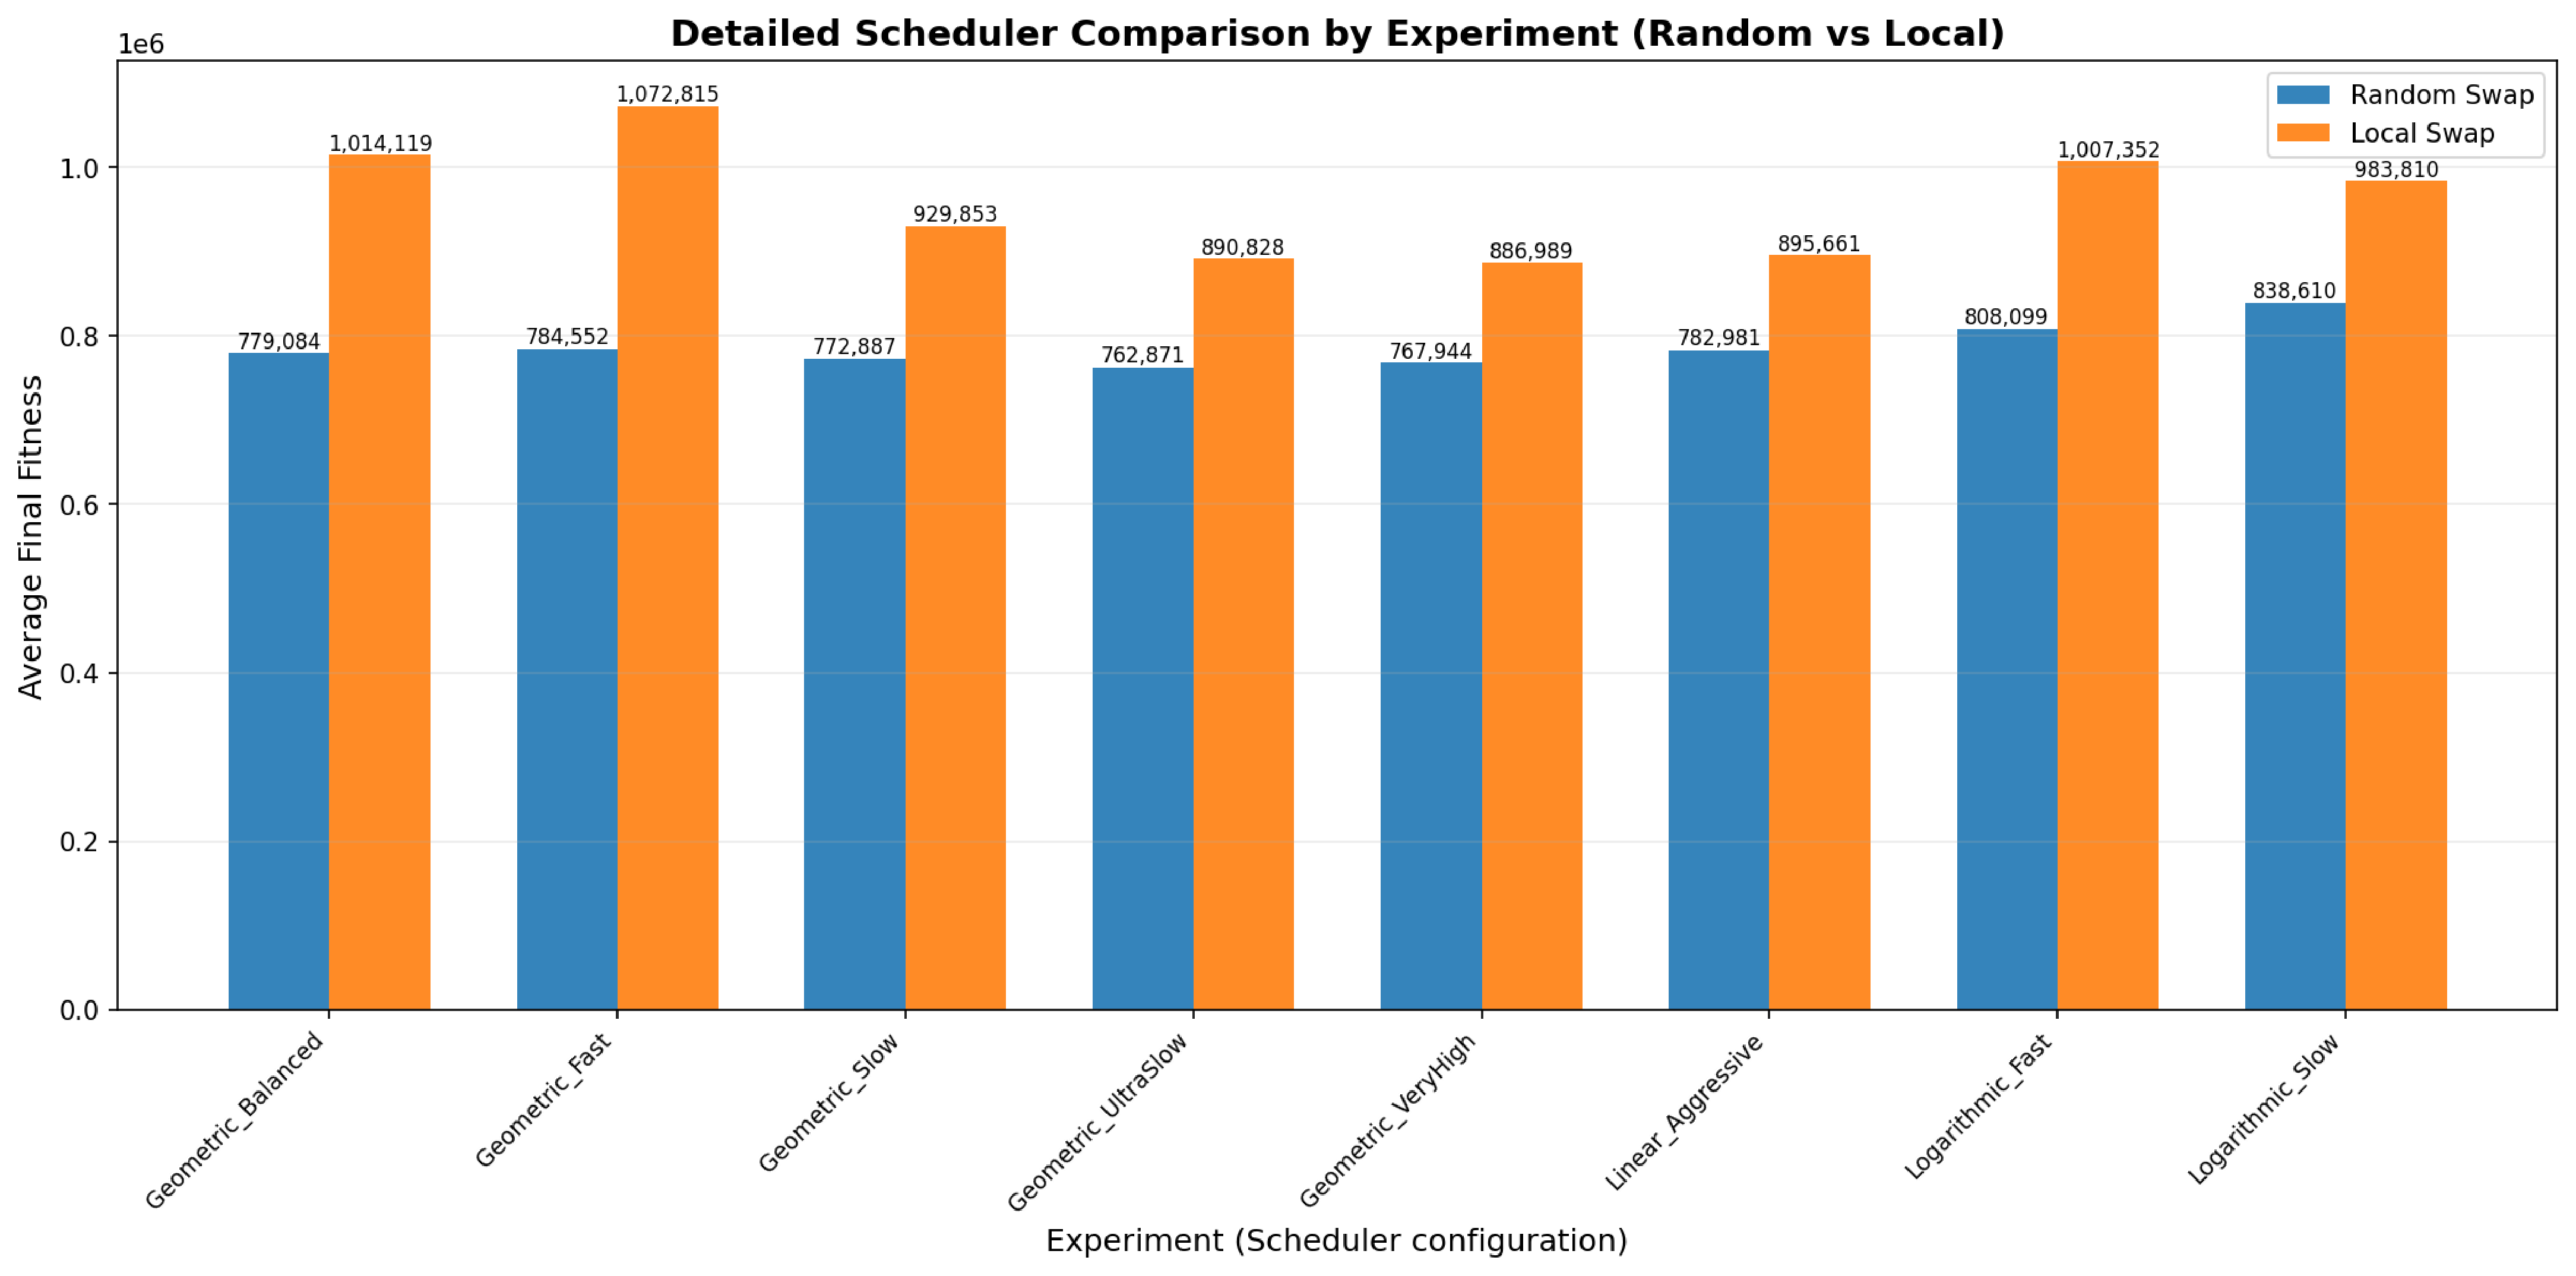
\includegraphics[width=0.65\textwidth]{recursos/moby_dick_scheduler_comparison_detailed.pdf}
  \end{center}
  
  
  \begin{center}
    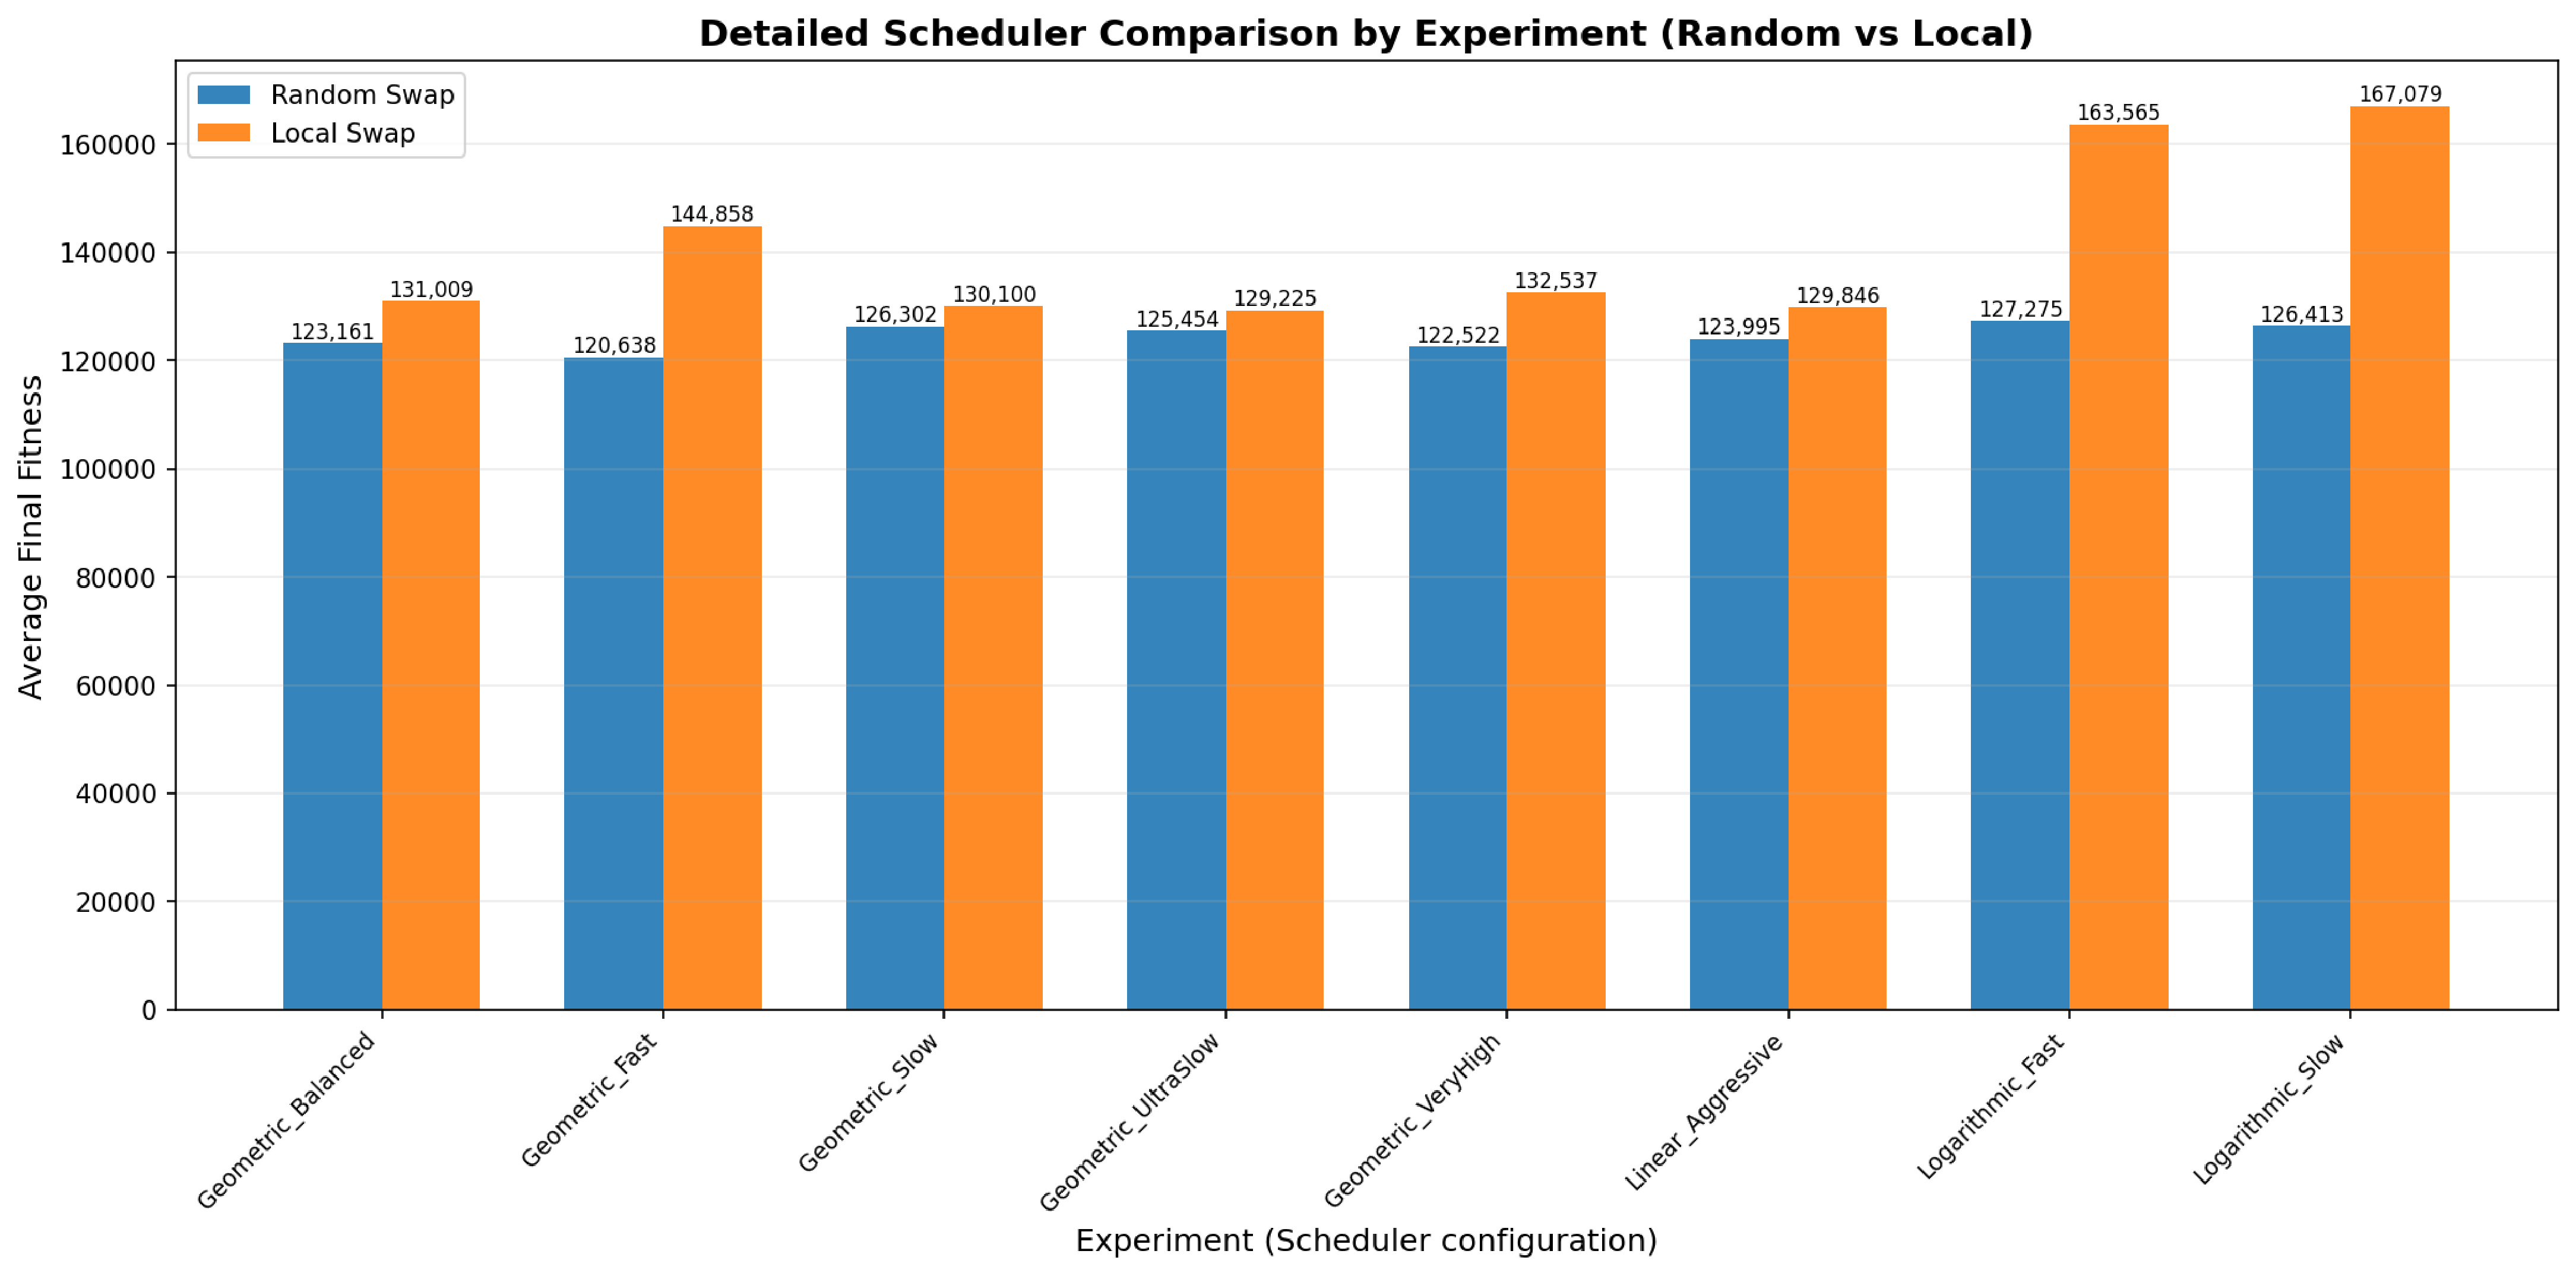
\includegraphics[width=0.60\textwidth]{recursos/wizard_oz_scheduler_comparison_detailed.pdf}
  \end{center}
\end{frame}

\begin{frame}{Experimentos Enfriamiento (II)}
  \begin{columns}[T]
    \begin{column}{0.48\textwidth}
      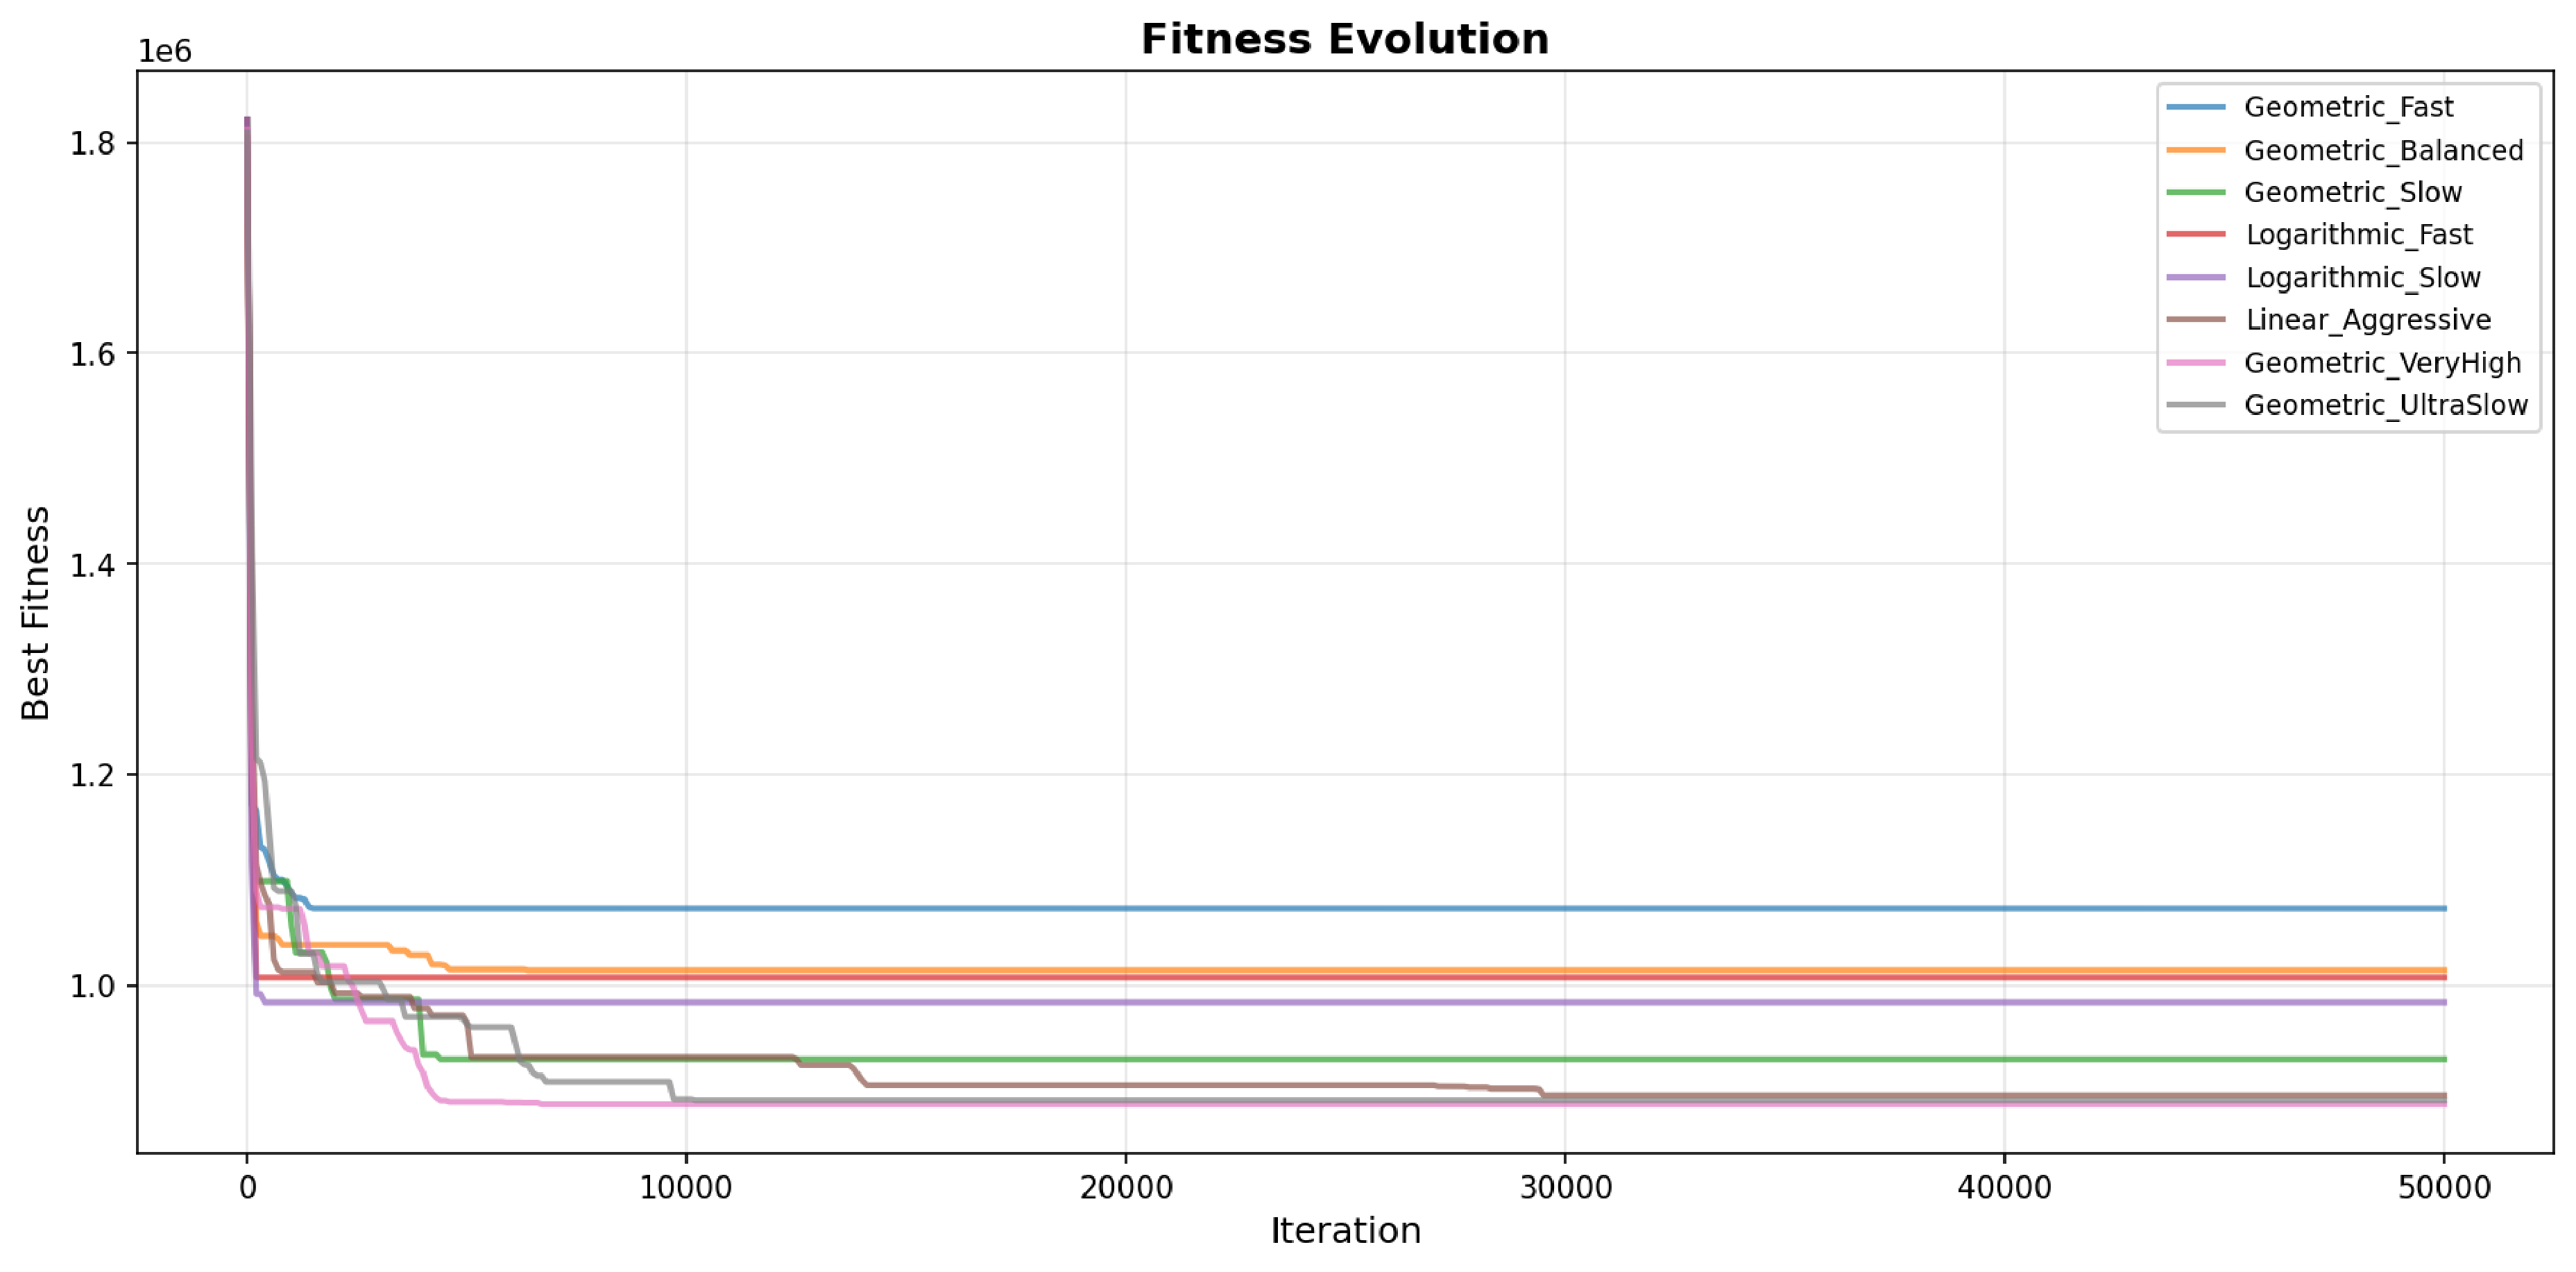
\includegraphics[width=\textwidth]{recursos/moby_dick_fitness_evolution_local.pdf}
      \vspace{0.3em}
      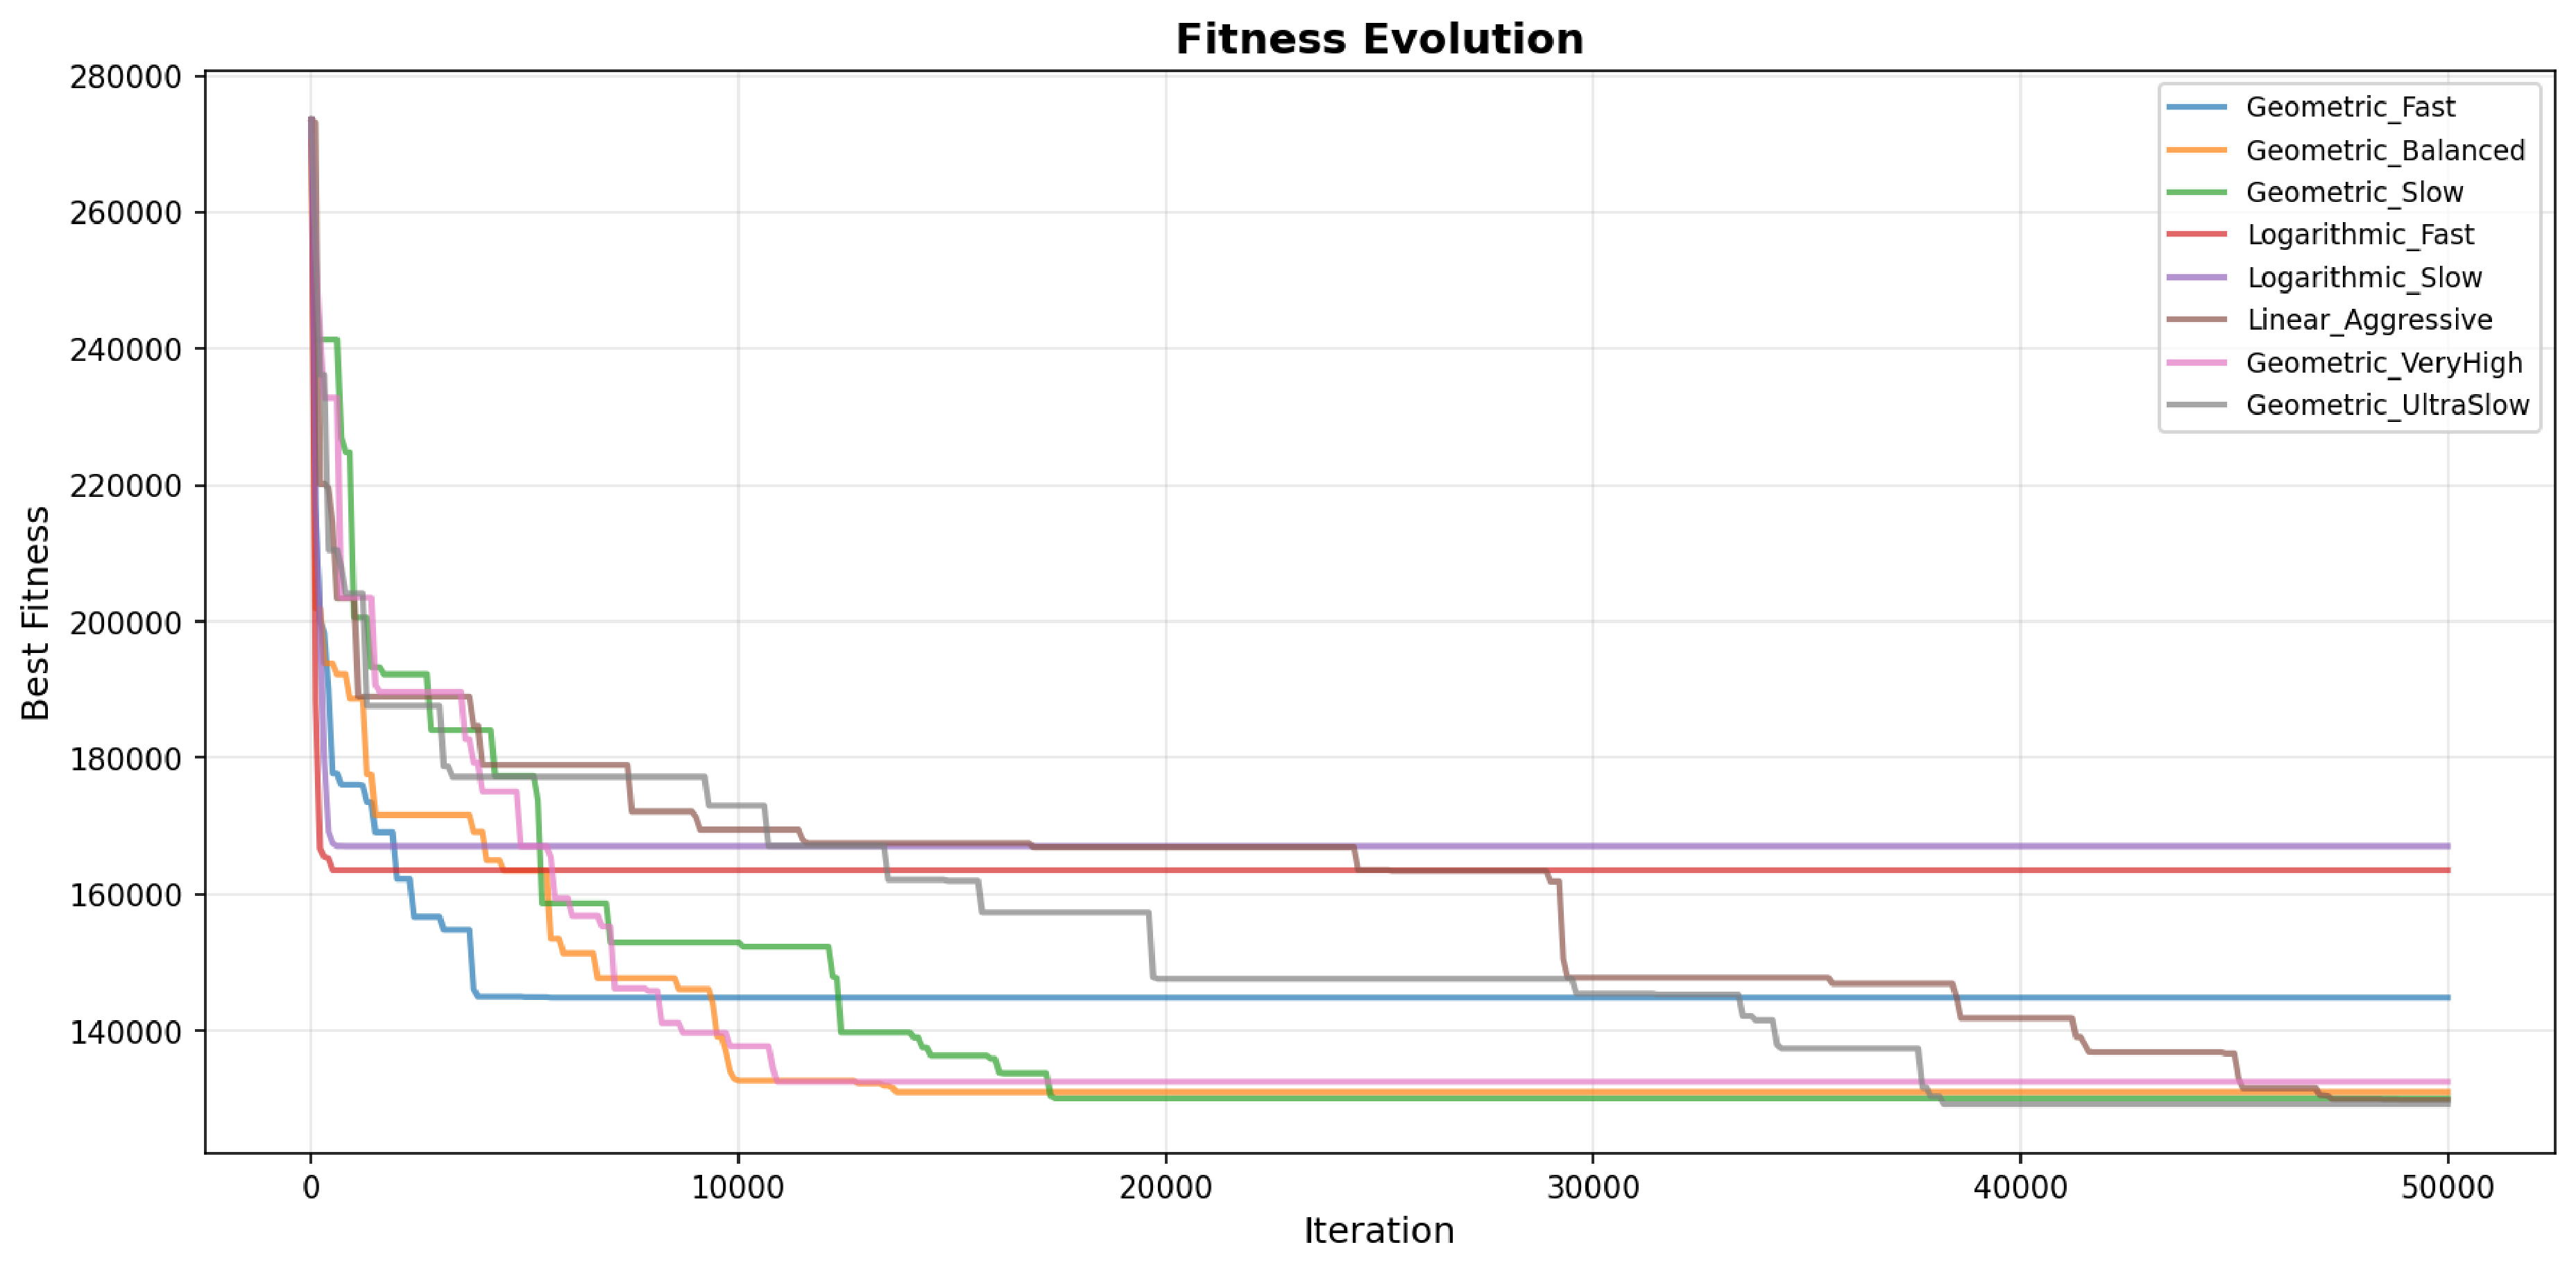
\includegraphics[width=\textwidth]{recursos/wizard_oz_fitness_evolution_local.pdf}
    \end{column}
    
    \begin{column}{0.48\textwidth}
      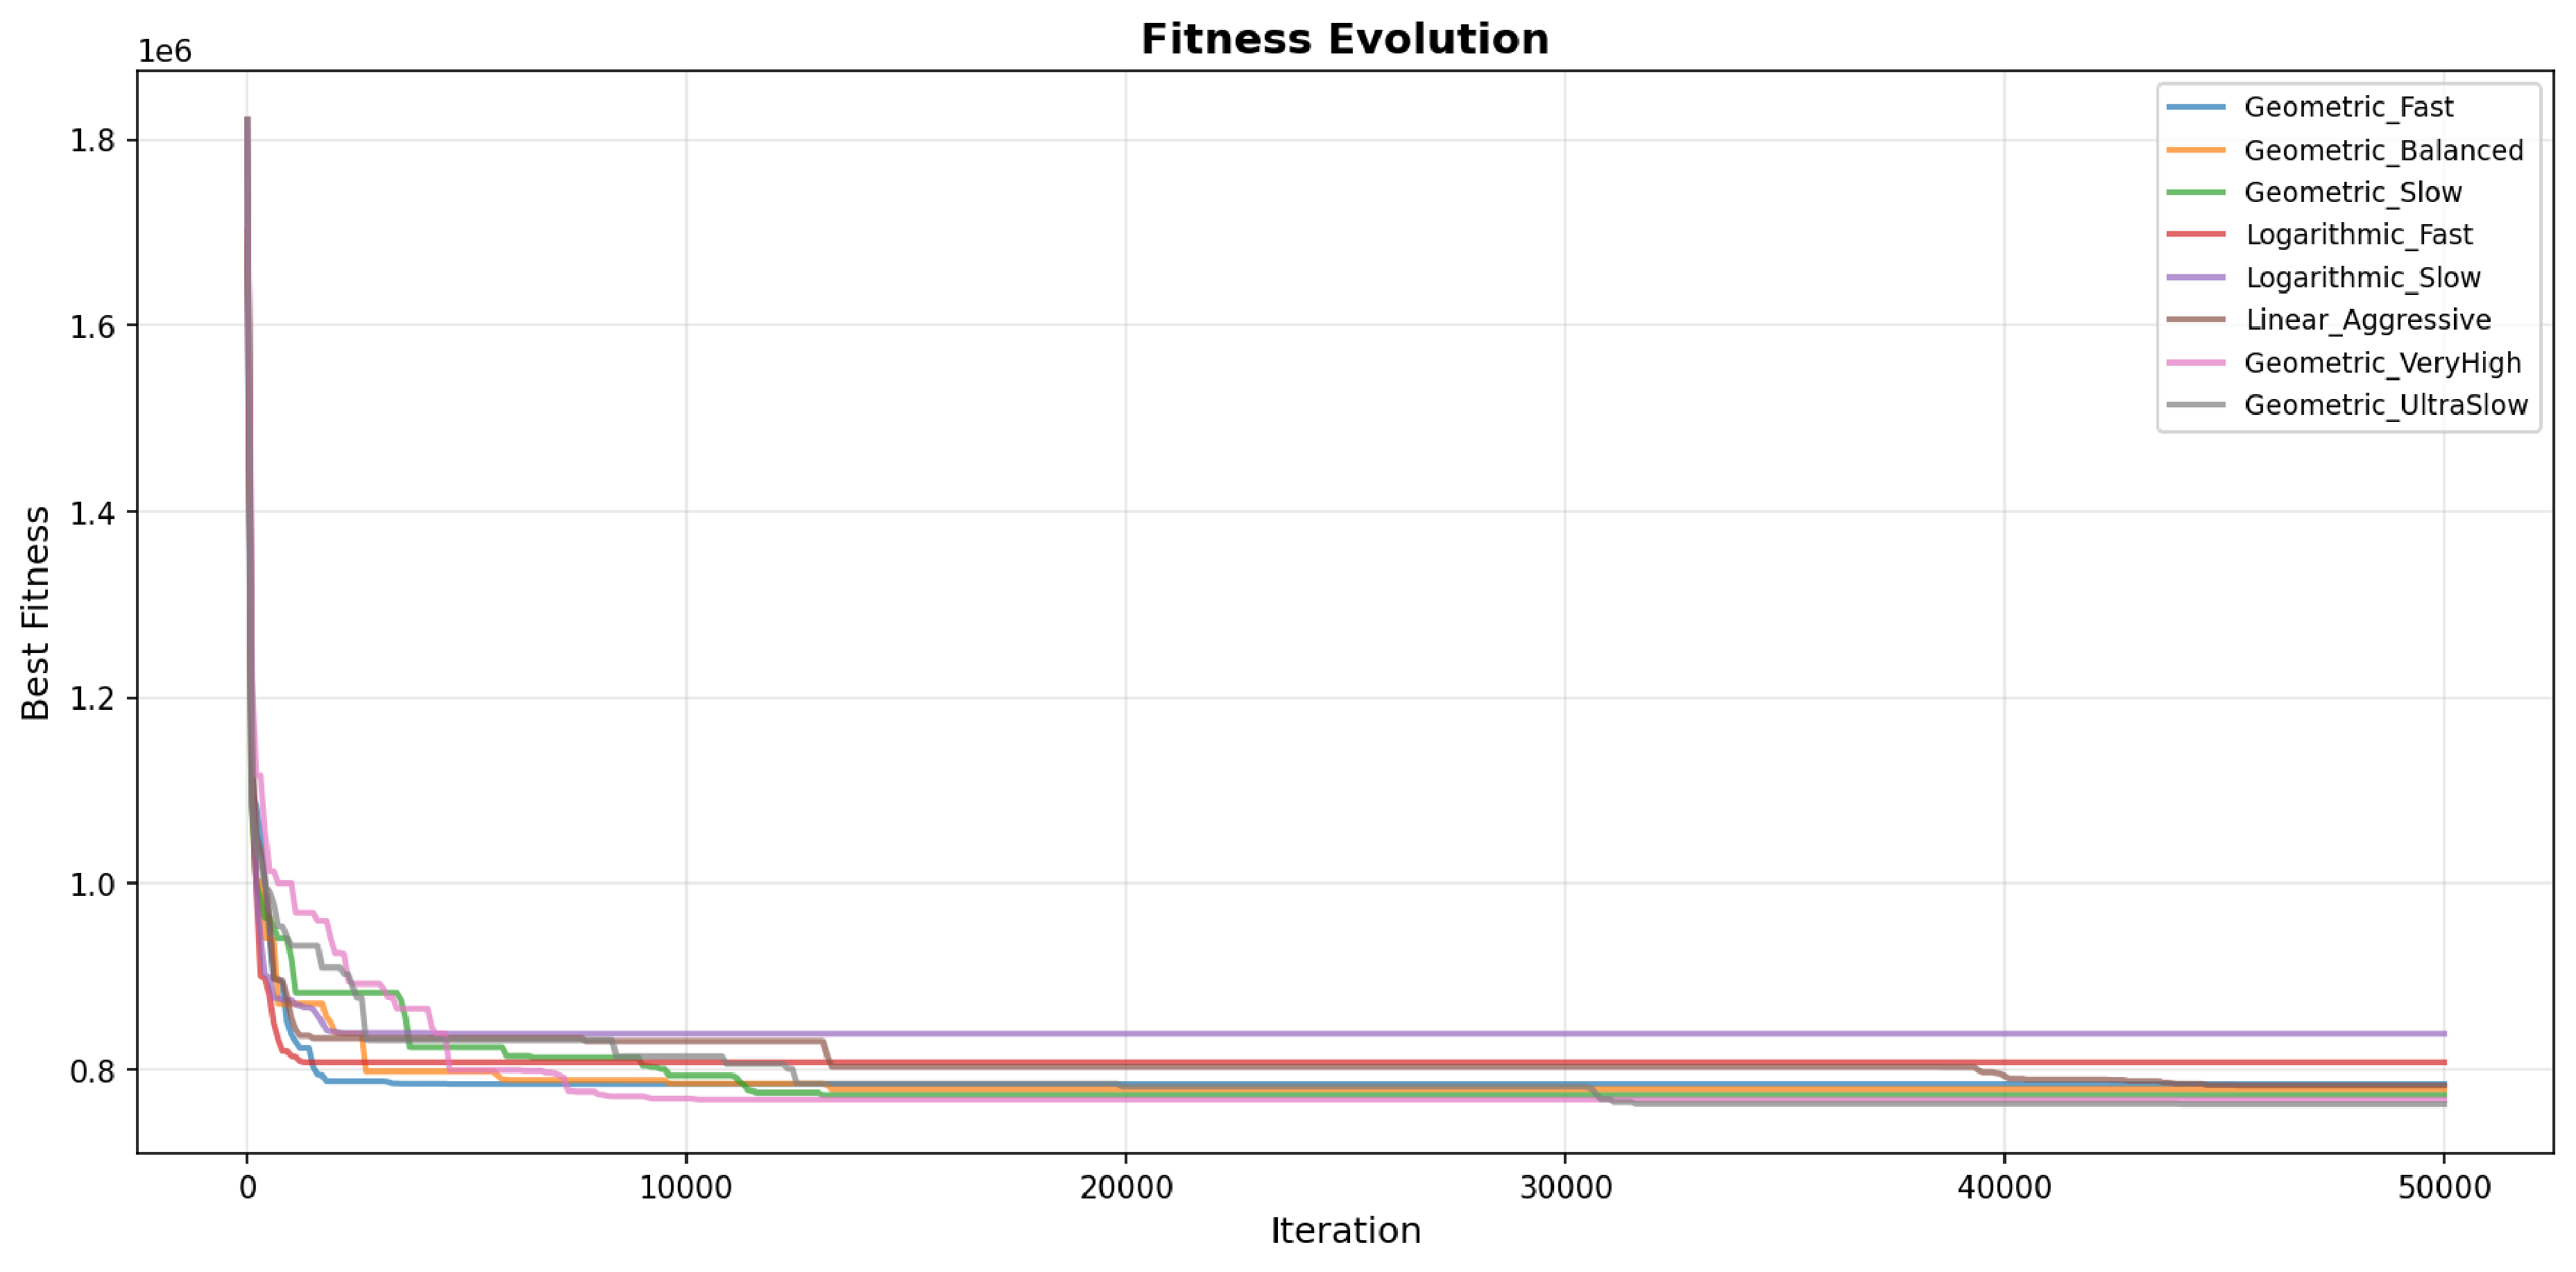
\includegraphics[width=\textwidth]{recursos/moby_dick_fitness_evolution_random.pdf}
      \vspace{0.3em}
      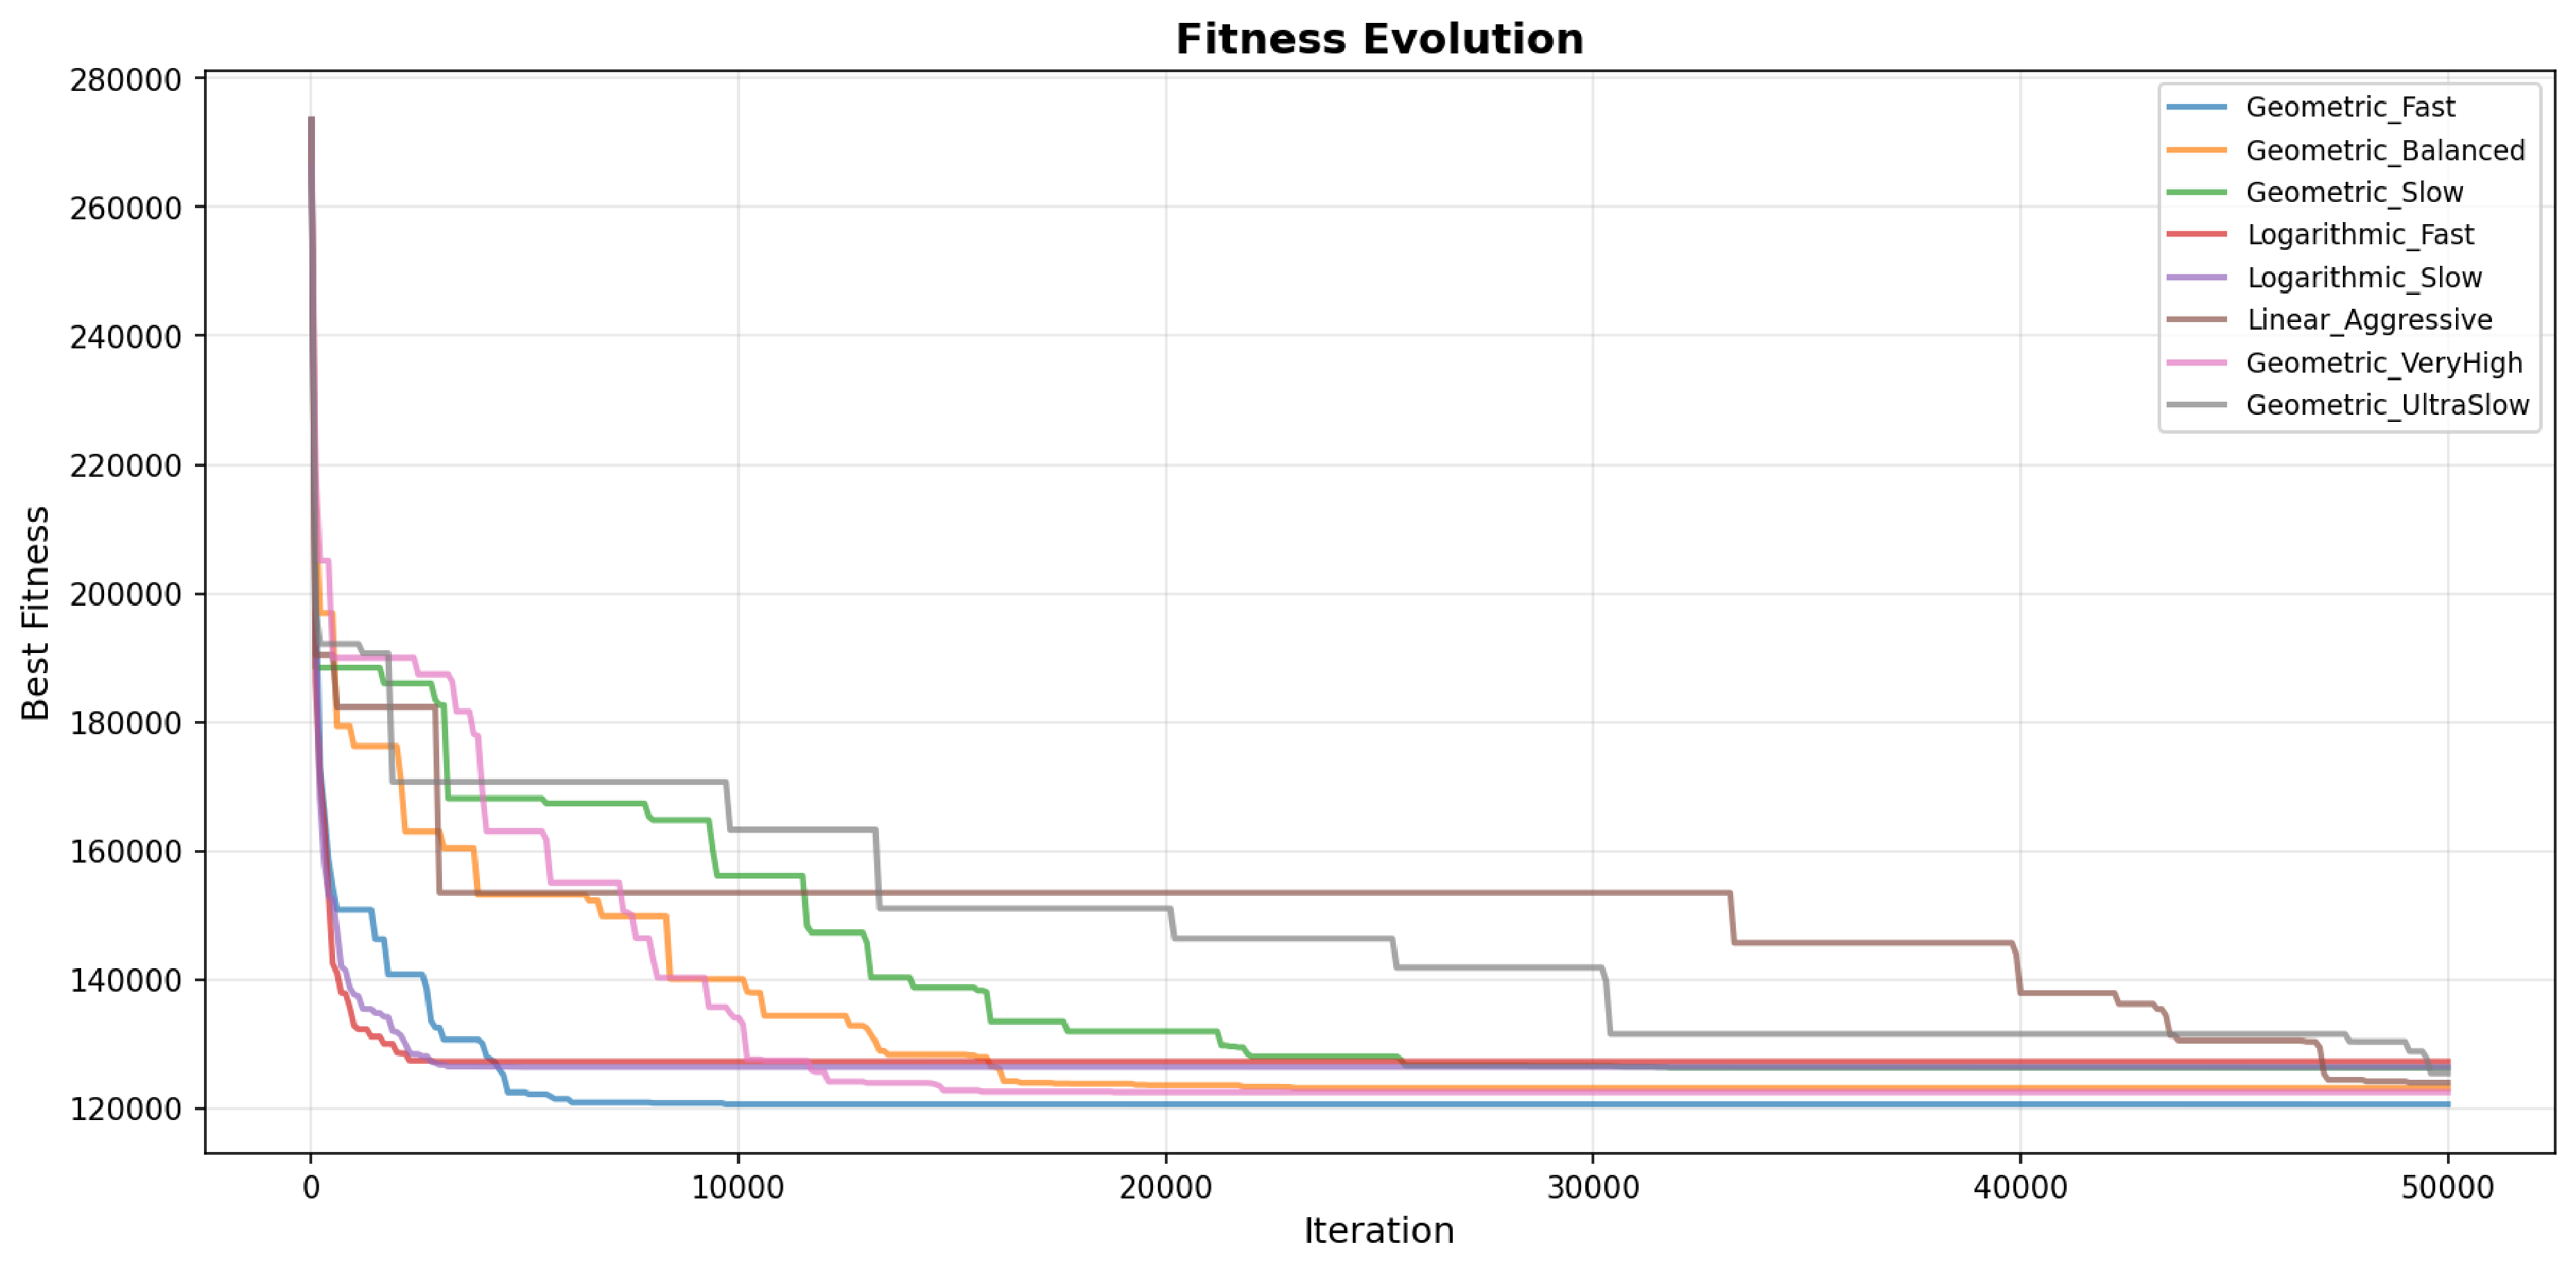
\includegraphics[width=\textwidth]{recursos/wizard_oz_fitness_evolution_random.pdf}
    \end{column}
  \end{columns}
\end{frame}



%% ============================================
%% SECCIÓN 5: CONCLUSIONES
%% ============================================
\section{Conclusiones}
\begin{frame}{Consideraciones finales}
  \begin{columns}[T]
    \begin{column}{0.48\textwidth}
      \begin{center}
        \textbf{Moby Dick (1.2M chars)}
        \vspace{0.3em}
        
        % Teclado centrado
        \begin{tikzpicture}[scale=0.55, every node/.style={transform shape}]
          \tikzstyle{key} = [rectangle, draw=ForestGreen!70!black, fill=green!20, 
            rounded corners=2pt, minimum width=0.75cm, minimum height=0.75cm, font=\small\bfseries]
          
          % Primera fila
          \foreach \letter [count=\i] in {Z,W,C,D,N,I,H,G,K,;}
            \node[key] at (\i*0.85-4.25, 3) {\letter};
          
          % Segunda fila (home row) - destacada
          \foreach \letter [count=\i] in {V,M,R,S,T,O,A,E,{,},{.}}
            \node[key, fill=green!40] at (\i*0.85-4.25, 2) {\letter};
          
          % Tercera fila
          \foreach \letter [count=\i] in {J,Q,B,F,L,U,P,Y,X,'}
            \node[key] at (\i*0.85-4.25, 1) {\letter};
        \end{tikzpicture}
      \end{center}
      
      \vspace{0.5em}
      
      \begin{beamercolorbox}[sep=6pt,center,rounded=true,shadow=true]{block body successful}
        \textbf{Fitness: 2,982.5}\\
        \small 65.0\% mejor que QWERTY
      \end{beamercolorbox}
      
      \vspace{0.3em}
      
    \end{column}
    
    \begin{column}{0.48\textwidth}
      \begin{center}
        \textbf{Wizard of Oz (0.3M chars)}
        \vspace{0.3em}
        
        % Teclado centrado
        \begin{tikzpicture}[scale=0.55, every node/.style={transform shape}]
          \tikzstyle{key} = [rectangle, draw=blue!70!black, fill=blue!20, 
            rounded corners=2pt, minimum width=0.75cm, minimum height=0.75cm, font=\small\bfseries]
          
          % Primera fila
          \foreach \letter [count=\i] in {',B,M,L,D,{,},Y,P,;,J}
            \node[key] at (\i*0.85-4.25, 3) {\letter};
          
          % Segunda fila (home row) - destacada
          \foreach \letter [count=\i] in {V,F,R,S,N,E,A,O,U,.}
            \node[key, fill=blue!40] at (\i*0.85-4.25, 2) {\letter};
          
          % Tercera fila
          \foreach \letter [count=\i] in {X,K,C,W,H,I,T,G,Z,Q}
            \node[key] at (\i*0.85-4.25, 1) {\letter};
        \end{tikzpicture}
      \end{center}
      
      \vspace{0.1em}
      
      \begin{beamercolorbox}[sep=6pt,center,rounded=true,shadow=true]{block body}
        \textbf{Fitness: 3,437.1}\\
        \small 59.7\% mejor que QWERTY
      \end{beamercolorbox}
      
      \vspace{0.3em}
      
    \end{column}
  \end{columns}

  \begin{block}{Conclusión}
    \begin{itemize}
      \item \textbf{AG →} mejor exploración; \textbf{ES →} mayor convergencia.
      \item Resultados estables y \textbf{generalizables} entre corpus.
      \item AG + ES híbrido \textbf{promete mejores resultados}.
      \item Layout para Moby Dick presenta mayor \textbf{generalización}.
    \end{itemize}
  \end{block}

\end{frame}

\begin{frame}{}
  \centering
  \vspace{2em}
  \Huge
  \textcolor{UPVBlue}{¡Gracias por vuestra atención!}
  
  \vspace{1em}
  
  \Large
  ¿Preguntas?
  
  \vspace{1em}
  
  \normalsize
  \faGithub\ GitHub:\\
  \small
  \texttt{github.com/JordiCan/}\\
  \texttt{hybrid-keyboard-optimizer}
  
  \vspace{1.5em}
  
  \normalsize
  \faKeyboard\ Recursos:\\
  \small
  \href{https://www.keybr.com/layouts}{\texttt{keybr.com/layouts}}
  
  \vspace{1.5em}
  
  \normalsize
  \faEnvelope\ Email:\\
  \small
  \texttt{jcanfer1@etsinf.upv.edu.es}
\end{frame}


\end{document}